\documentclass[letterpaper,12pt,fleqn]{article}
\usepackage{matharticle}
\usepackage{tikz}
\pagestyle{plain}
\newcommand{\fillin}{\rule{3in}{1pt}}
\begin{document}

\begin{center}
\Large Math-19 Exam \#3
\end{center}

\vspace{0.5in}

Name: \rule{4in}{1pt}

\vspace{0.5in}

This exam is closed book and notes. You may use a calculator; however, no cell
phones or tablets are allowed. Show all work; there is no credit for guessed
answers. All values should be exact unless you are specifically asked for an
approximate value answer. In particular, trig answers should be left in terms
of $\pi$ unless otherwise directed.

\vspace{0.5in}

\begin{enumerate}
\item Identify the following formulas. Be specific regarding orientation.
  
  \begin{tabular}{cc}
    \\
    $\frac{\sin{A}}{a}=\frac{\sin{B}}{b}=\frac{\sin{C}}{c}$ & \fillin \\
    \\
    $c^2=a^2+b^2-2ab\cos\theta$ & \fillin \\
    \\
    $Ax^2+Bxy+Cy^2+Dx+Ey+F=0$ & \fillin \\
    \\
    $(x-h)^2=4p(y-k)$ & \fillin \\
    \\
    $(y-k)^2=4p(x-h)$ & \fillin \\
    \\
    $(x-h)^2+(y-k)^2=r^2$ & \fillin \\
    \\
    $\frac{(x-h)^2}{a^2}+\frac{(y-k)^2}{b^2}=1$ & \fillin \\
    \\
    $\frac{(y-k)^2}{a^2}+\frac{(x-h)^2}{b^2}=1$ & \fillin \\
    \\
    $\frac{(x-h)^2}{a^2}-\frac{(y-k)^2}{b^2}=1$ & \fillin \\
    \\
    $\frac{(y-k)^2}{a^2}-\frac{(x-h)^2}{b^2}=1$ & \fillin \\
  \end{tabular}
\newpage
\item Consider the following trigonometric function:
  \[y=-2\cos(2\pi x-\frac{\pi}{2})\]
  \begin{enumerate}
  \item What is the amplitude (A)?

    \vspace{1in}
    
  \item What is the period (P)?

    \vspace{1in}
    
  \item What is the horizontal translation (b)?

    \vspace{1in}
    
  \item Sketch one period of the function on the interval $[b,b+P]$.
  \end{enumerate}
\newpage
\item The following problem asks you to derive various trigonometric
  identities, starting from the cosine addition formula.
  \begin{enumerate}
  \item State the cosine addition formula.

    \vspace{1in}
    
  \item State the cosine subtraction formula (hint: even/odd).

    \vspace{1in}
    
  \item Derive the sine addition formula (hint: cofunction identity).

    \vspace{2in}
    
  \item Derive the sine subtraction formula (hint: even/odd).

    \vspace{1in}
    
  \item Derive the $\cos{x}\sin{y}$ sum to product formula.

   \vspace{3in}

  \end{enumerate}

\item Find an exact value for $\cos105^{\circ}$.

  \vspace{2in}

\item State the cos/sin version of the pythagorean identity and then
  derive the other two forms (tan/sec and cot/csc).

  \vspace{3in}

\item Prove the following identity:
  \[\frac{1}{\sec{x}-\tan{x}}-\frac{1}{\sec{x}+\tan{x}}=2\tan{x}\]

  \vspace{3in}

\item Find all solutions.
  \[\cos^2\left(\frac{x}{2}\right)=\frac{3}{4}\]

  \vspace{4in}
  
\item Write as a function of $x$:
  \[\sin\left(\cos^{-1}x+\sin^{-1}x\right)\]
\newpage
\item A 10-foot pole is suspended against a building such that the bottom of
  the pole is where the building meets the ground and the top of the pole is
  connected by a rope to a hook that is 12 feet up on the side on the building.
  The angle the pole makes with the ground is $60^{\circ}$.

  \begin{center}
  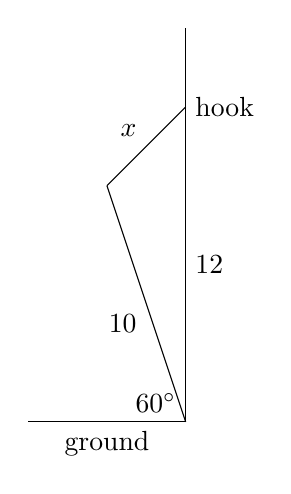
\begin{tikzpicture}
    \draw (0,0) -- (2,0);
    \draw (2,0) -- (2,5);
    \draw (2,0) -- (1,3);
    \draw (1,3) -- (2,4);
    \node [below] at (1,0) {ground};
    \node [right] at (2,4) {hook};
    \node [left] at (1.5,1.25) {$10$};
    \node [right] at (2,2) {$12$};
    \node [above left] at (2,0) {$60^{\circ}$};
    \node [above left] at (1.5,3.5) {$x$};
  \end{tikzpicture}
  \end{center}

  What is the length $x$ of the rope, accurate to one decimal place?

  \vspace{3in}

\item Consider the following equation:
  \[x^2+4y^2-2x+16y+13=0\]
  \begin{enumerate}
  \item Explain how by looking at the equation you can tell that this is an
    ellipse.

    \vspace{2in}
    
  \item Put the equation in standard form.

    \vspace{4in}

  \item What are the coordinates of the center?

    \vspace{1in}
  
  \item What is $a$?

    \vspace{1in}
  
  \item What is $b$?

    \newpage
  
  \item What is $c$?

    \vspace{2in}
  
  \item What are the four vertices?

    \vspace {1in}
    
  \item What are the two foci?

    \vspace {1in}

  \item Sketch the ellipse. Be sure to label all of the above values.
  \end{enumerate}
\end{enumerate}
\end{document}
